\documentclass[10pt,varwidth]{standalone}
\usepackage[a4paper, left=2.5cm, right=2.5cm, top=2.5cm, bottom=2.5cm]{geometry}
\usepackage{xifthen}
\usepackage{xfp}
\usepackage{xcolor}
\usepackage{pgfplots}
\usepackage{pgfplotstable}
\pgfplotsset{compat=1.16}
% 2.引用的tikz库
\usetikzlibrary {matrix, chains, trees, decorations}
\usetikzlibrary {arrows.meta, automata,positioning}
\usetikzlibrary {decorations.pathmorphing, calc}
\usetikzlibrary {calligraphy}
\usetikzlibrary {backgrounds, mindmap,shadows}
\usetikzlibrary {patterns, quotes, 3d, shadows}
\usetikzlibrary {graphs, fadings, scopes}
\usetikzlibrary {arrows, shapes.geometric}
\usepgflibrary {shadings}

\tikzset{
    >={Latex[length=6mm, width=2mm]}
}



\begin{document}
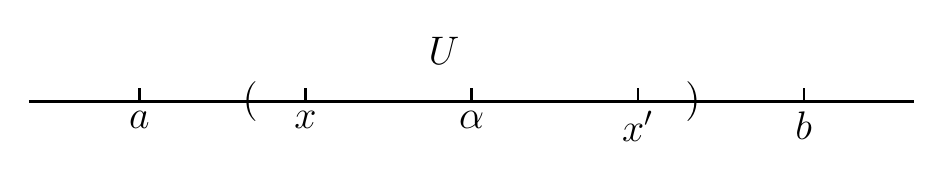
\begin{tikzpicture}[font=\Large]
    \draw[thick] (-16em, 0) -- (16em, 0);
    \node[below] at (6em, 0) {$x'$}; 
    \node[below] at (12em, 0) {$b$}; 
    \node[below] at (0em, 0) {$\alpha$}; 
    \node[below] at (-6em, 0) {$x$}; 
    \node[below] at (-12em, 0) {$a$}; 
    \node[above] at (-1em, 1em) {$U$}; 
    \node at (-8em, 0) {$\mathbf{(}$};
    \node at (8em, 0) {$\mathbf{)}$};
    \foreach \i in {-12em, -6em, 0, 6em, 12em}{
        \draw[thick] (\i, 0) -- (\i, .5em);
    }
\end{tikzpicture}
\end{document}